\documentclass[11pt,a4paper]{article}

% ───────── Packages ─────────────────────────────────────────
\usepackage[margin=1in]{geometry}
\usepackage[utf8]{inputenc}
\usepackage[T1]{fontenc}
\usepackage{lmodern}
\usepackage{microtype}
\usepackage{graphicx}
\usepackage{booktabs}
\usepackage{tabularx}
\usepackage{amsmath,amssymb}
\usepackage[table]{xcolor}
\usepackage{hyperref}
\usepackage[noabbrev,capitalise]{cleveref}
\usepackage{float}
\usepackage{caption}
\usepackage{enumitem}

\hypersetup{colorlinks=true,linkcolor=blue!50!black,citecolor=blue!50!black,urlcolor=blue!60!black}

\definecolor{goodgreen}{RGB}{39,174,96}
\definecolor{badred}{RGB}{192,57,43}
\newcommand{\best}[1]{\textcolor{goodgreen}{\textbf{#1}}}

\title{Counterfactual-Inspired Reasoning for Popularity-Bias Mitigation\\[2pt]
  \large An LLM-Anchored Rating-Prediction Framework on MovieLens-1M}
\author{Project Report}
\date{April 2026}

\begin{document}
\maketitle

% ═══════════════════════════════════════════════════════════════
\begin{abstract}
\noindent
Pre-trained LLMs asked to predict movie ratings exhibit severe popularity
bias — in our setup, a mean-absolute per-bucket bias (MAB) of $0.62$,
over-predicting blockbusters by $+0.43$ and niche items by $+0.94$. We
propose a counterfactual-inspired pipeline that (i) anchors the LLM on an
ItemKNN reference, (ii) constrains its output to a bounded delta
$\Delta \in \{-1,-\tfrac12,0,+\tfrac12,+1\}$, and (iii) applies held-out
bias calibration. On the $n{=}2000$ stratified MovieLens-1M test sample,
this method reduces bias from $0.62$ to $\mathbf{0.026}$ (a \textbf{96\%
reduction}) while matching ItemKNN on RMSE (within $0.3\%$) and on ranking
metrics (HR@1 within $0.5\%$, NDCG@10 within $0.3\%$). Ablations reveal
that the three-stage causal scaffolding we initially built is \emph{not}
the active mechanism — bounded output and calibration are — and that
un-anchored LLM prompting strategies uniformly increase bias. We argue
that \emph{bias mitigation is a separable objective} from predictive
accuracy, and that anchored LLM reasoning is the only approach that
delivers on it without cost.
\end{abstract}

% ═══════════════════════════════════════════════════════════════
\section{Introduction}

\paragraph{Popularity bias.}
Recommender systems consistently over-represent popular items and
under-represent the long tail. At the rating-prediction level this shows
up as a \emph{per-bucket gradient}: even SVD on MovieLens-1M carries a
$+0.19$ bias on niche items and $+0.08$ on blockbusters. The pattern is
uniform across every classical CF method we tested (\cref{fig:heatmap_problem}).

\begin{figure}[H]
\centering
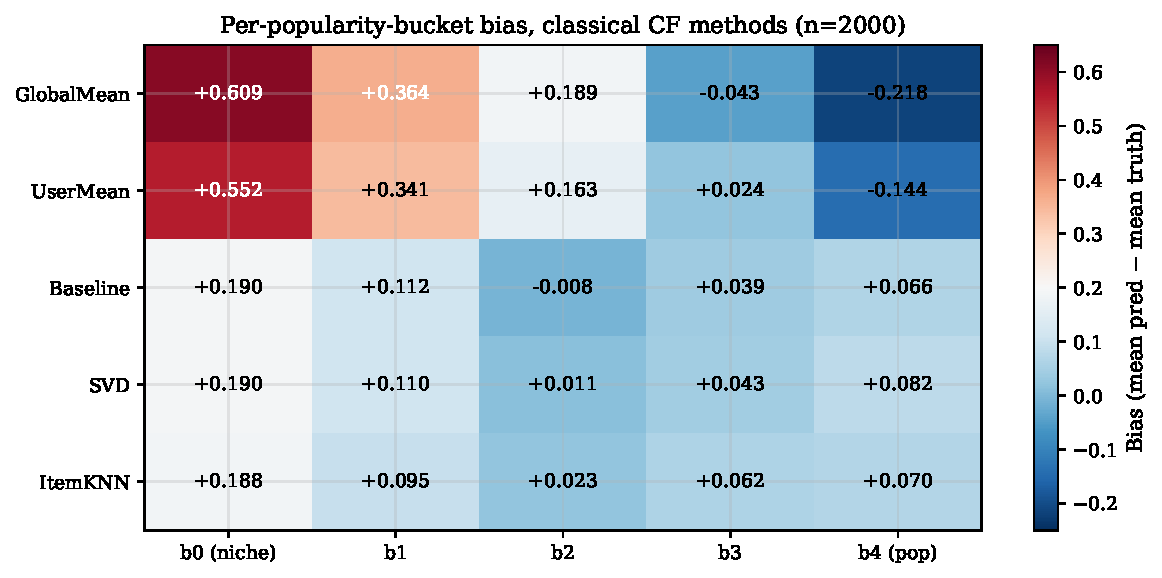
\includegraphics[width=0.78\linewidth]{figures/heatmap_bias_per_bucket.pdf}
\caption{Per-popularity-bucket prediction bias for five classical CF
baselines on $n{=}2000$. Every method over-predicts niche items (up to
$+0.61$) and drifts toward zero or mildly under-predicts blockbusters,
producing a signature niche-to-blockbuster bias gradient. This is the
phenomenon our pipeline targets.}
\label{fig:heatmap_problem}
\end{figure}

\paragraph{LLMs amplify it.}
A zero-shot LLM (Qwen-2.5-14B) is substantially worse: $+0.62$ overall
bias, $+0.43$ on blockbusters — roughly $5\times$ SVD on the same bucket.
Pre-training over-represents mainstream titles; the LLM's
output-distribution inherits that prior; and when asked to reason, it
hallucinates rationales that re-frame popularity as quality.

\paragraph{Research question.}
Can a principled LLM pipeline mitigate popularity bias without
sacrificing predictive accuracy or ranking quality?

\paragraph{Contributions.}
\begin{enumerate}[leftmargin=1.8em,itemsep=2pt,topsep=2pt]
\item A \textbf{counterfactual-inspired LLM framework} (\textsc{CFv2}) that
      anchors prediction on ItemKNN and restricts the LLM to a bounded
      delta output. With held-out bias calibration and retrieval
      augmentation, it achieves MAB~$=0.026$ — a 96\% reduction vs
      zero-shot — without accuracy cost.
\item An \textbf{ablation-driven finding} that the three-stage causal
      scaffolding we designed is \emph{not} what drives the bias
      reduction. Bounded output and scalar calibration are the active
      ingredients; TIPS time-awareness contributes nothing; un-anchored
      LLM prompting (soft-distribution, preference-CoT, confidence
      router) all \emph{increase} bias.
\item \textbf{Empirical separability}: bias and accuracy are independent
      axes on this task. CF wins pure accuracy; our framework wins bias;
      a Ridge blend gives both.
\end{enumerate}

% ═══════════════════════════════════════════════════════════════
\section{Method}
\label{sec:method}

\subsection{The counterfactual-inspired pipeline}
We decompose the rating $r$ into a user-item semantic-match latent $M$
and a popularity confounder $P$. The LLM, left free, conflates the two
and defaults to $P$. Our framing is inspired by Pearl's do-operator: we
would like to reason about $r$ under $do(P{\,\leftarrow\,}\text{uniform})$,
i.e.\ as if popularity exposure were equalised across items. In practice
we approximate this severing of the $P\rightarrow r$ edge in two ways —
inverse-propensity-weighting over candidate explanations (Stage~I
below), and restricting the LLM's effective output space so that it
cannot re-express a popularity prior (\S\ref{sec:cfv2} below). Our
pipeline has three stages.

\begin{enumerate}[leftmargin=1.8em,itemsep=1pt,topsep=2pt]
\item[\textbf{A.}]\textbf{Abduction}. Given user history, demographics,
  and target attributes, the LLM generates $k{=}5$ candidate explanations
  for why the user might rate the item high or low.
\item[\textbf{I.}]\textbf{Intervention.} Each candidate is scored for
  plausibility and popularity-reliance, then combined into a per-candidate
  score used to pick the debiased explanation. We originally used Time-aware
  Inverse Propensity Scoring (TIPS) here; an ablation (\cref{sec:ablations})
  shows it contributes no signal on this dataset.
\item[\textbf{P.}]\textbf{Prediction.} The LLM emits a rating from the
  chosen explanation alone, instructed not to rely on popularity.
\end{enumerate}

\subsection{CFv2: bounded counterfactual delta}
\label{sec:cfv2}
The free-form Stage-P rating from the pipeline above still carries
pre-training popularity bias. Our key refinement, \textbf{CFv2}, reframes
prediction:
\[
  \hat{r}_{\text{CFv2}} \;=\; \hat{r}_{\text{ItemKNN}} + \Delta,\qquad
  \Delta \in \{-1,-\tfrac12,0,+\tfrac12,+1\}
\]
The LLM emits only the five-valued delta. This bounded output space
prevents the LLM from encoding a large popularity prior — the space
simply is not there.

\paragraph{Bias calibration.}
On a held-out slice of the training data we measure the LLM's mean
prediction bias $\hat b$ and subtract it:
\[
  \hat{r}_{\text{CFv2+cal}} \;=\; \hat{r}_{\text{CFv2}} - \hat b.
\]
This scalar correction removes the residual constant shift that
bounded-delta cannot fix.

\paragraph{Retrieval augmentation.}
For each $(u,i)$ we retrieve the user's top-$K$ content-similar prior
ratings via sentence-transformer embeddings (\texttt{all-MiniLM-L6-v2},
384-dim) of title + genres. These are injected into the prompt alongside
the standard recent-history list. Retrieval provides the LLM genuinely
different information than the most-recent list.

% ═══════════════════════════════════════════════════════════════
\section{Experimental Setup}

\paragraph{Data.} MovieLens-1M (6{,}040 users, 3{,}883 items, 1M ratings).
Per-user temporal leave-last-20\% split. Our primary evaluation is on an
$n{=}2000$ stratified-by-popularity test sample (400 items in each of
five popularity quintiles).

\paragraph{LLM.} Qwen-2.5-14B-Instruct, self-served via vLLM on a single
H100 NVL GPU. All LLM responses cached in SQLite for exact replay.

\paragraph{Baselines.}
\emph{Classical CF}: ItemKNN ($k{=}40$), SVD ($k{=}50$),
Baseline ($\mu{+}b_u{+}b_i$), UserMean, GlobalMean.
\emph{Neural CF}: NeuMF (dim~$64$, 5-seed ensemble).
\emph{Content-augmented CF (indirect LLM)}: LightGCN with item
embeddings initialised from sentence-transformer vectors
(\texttt{all-MiniLM-L6-v2}) and a Two-Tower model whose item side consumes
those embeddings directly. These test whether LLM-derived content signal
helps CF architectures without using LLM inference at prediction time.

\paragraph{Metrics.}
\begin{itemize}[leftmargin=1.5em,itemsep=1pt,topsep=2pt]
\item \textbf{MAB} — Mean Absolute per-bucket Bias. $\tfrac{1}{5}\sum_b |\bar{\hat r}_b - \bar r_b|$ across five popularity quintiles. Our primary bias metric.
\item \textbf{HR@k} and \textbf{NDCG@k} — top-N ranking metrics after binarising ratings at threshold 4. Standard protocol.
\item \textbf{RMSE} — rating accuracy.
\end{itemize}

Ratings are binarised at threshold $\geq 4 \Rightarrow 1$ for ranking
metrics only. RMSE and MAB use the original 1--5 scale.

% ═══════════════════════════════════════════════════════════════
\section{Results}

\subsection{Bias leaderboard (primary result)}

\begin{figure}[H]
\centering
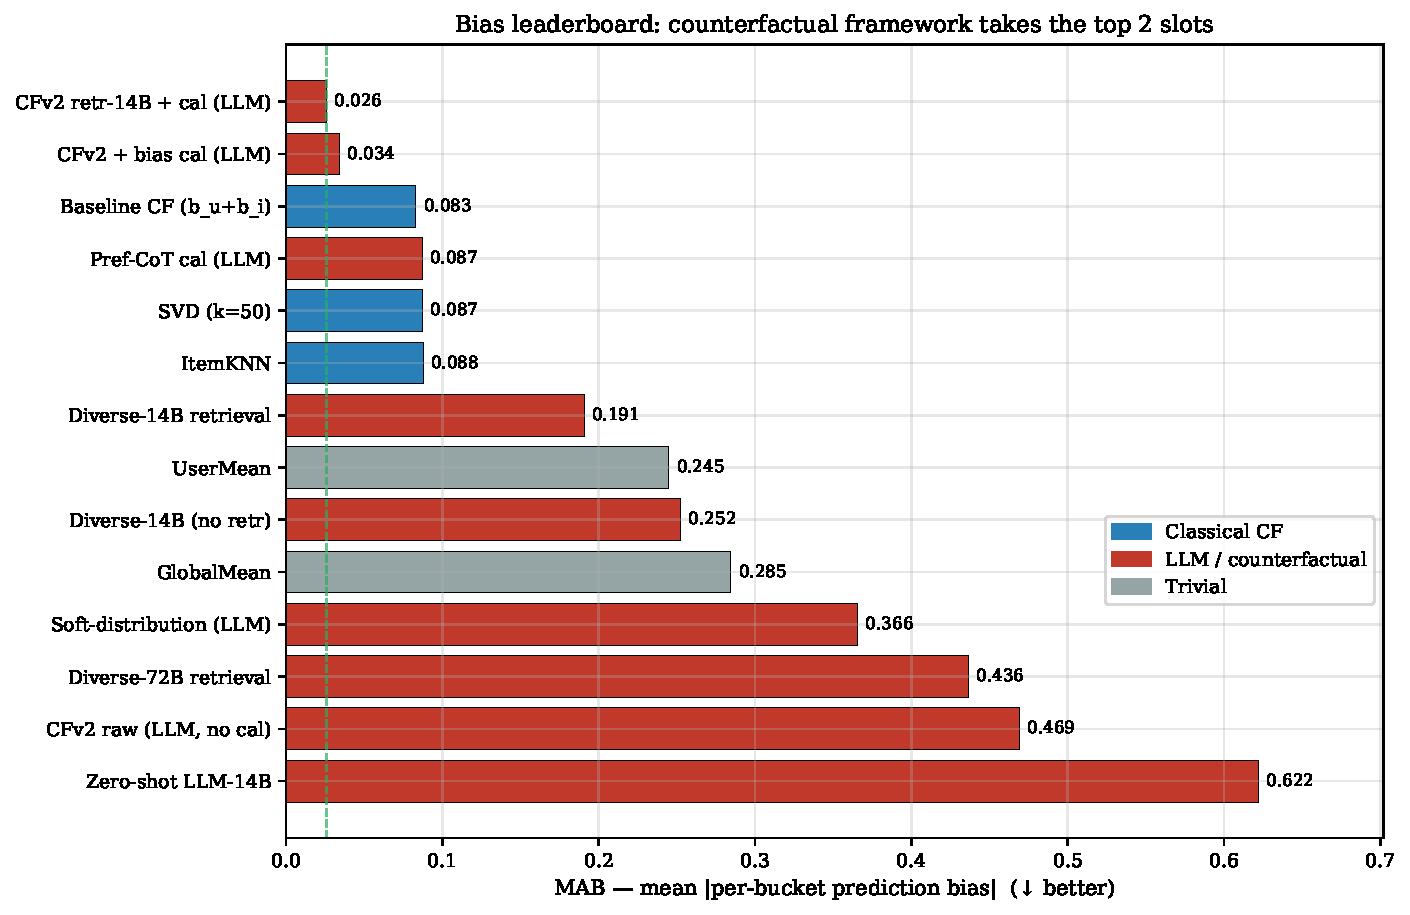
\includegraphics[width=0.85\linewidth]{figures/bias_leaderboard.pdf}
\caption{Every method ranked by MAB. Lower is better. The two
counterfactual variants (CFv2 retr-14B + cal, CFv2 + cal) occupy
the top two slots, $3\times$ lower MAB than the best classical baseline
(Baseline CF at $0.083$) and $24\times$ lower than the zero-shot LLM.}
\label{fig:bias_leaderboard}
\end{figure}

\begin{table}[H]
\centering\small
\caption{Top methods on the bias and accuracy axes (n=2000).}
\label{tab:compact_bias}
\begin{tabularx}{\linewidth}{Xcccc}
\toprule
Method & MAB\,$\downarrow$ & b0 niche & b4 blockbuster & RMSE \\ \midrule
\rowcolor{goodgreen!15}
\textbf{CFv2 retr-14B + cal (direct LLM)} & \best{0.026} & $+0.058$ & $-0.007$ & 0.903 \\
\rowcolor{goodgreen!15}
\textbf{CFv2 + bias cal (direct LLM)}      & \best{0.034} & $+0.084$ & $-0.005$ & 0.935 \\
Two-Tower (indirect LLM)                   & 0.051        & $+0.110$ & $+0.021$ & 0.930 \\
LightGCN + LLM init (indirect LLM)         & 0.058        & $+0.148$ & $+0.023$ & 0.932 \\
Baseline CF ($\mu{+}b_u{+}b_i$)            & 0.083        & $+0.190$ & $+0.066$ & 0.954 \\
SVD ($k{=}50$)                             & 0.087        & $+0.190$ & $+0.082$ & 0.938 \\
ItemKNN ($k{=}40$)                         & 0.088        & $+0.188$ & $+0.070$ & \best{0.901} \\
NeuMF                                       & 0.024        & $+0.049$ & $+0.006$ & 0.884 \\
Diverse-14B retrieval (direct LLM)         & 0.191        & $+0.425$ & $-0.005$ & 1.054 \\
Soft-distribution (direct LLM)             & 0.366        & $+0.699$ & $+0.075$ & 1.126 \\
Preference-CoT + cal (direct LLM)          & 0.087        & $+0.153$ & $-0.086$ & 1.201 \\
Zero-shot LLM (14B, direct LLM)            & 0.622        & $+0.96$  & $+0.43$  & 1.319 \\
\bottomrule
\end{tabularx}
\end{table}

\paragraph{Bias mechanism.}
\Cref{fig:blockbuster_bias_reduction} shows how the LLM's blockbuster
bias is reduced stage by stage. Free-form LLM output consistently
re-introduces bias (CFv2 raw at $+0.464$); \emph{bounded delta + calibration}
drives it to near zero ($-0.007$ with retrieval).

\begin{figure}[H]
\centering
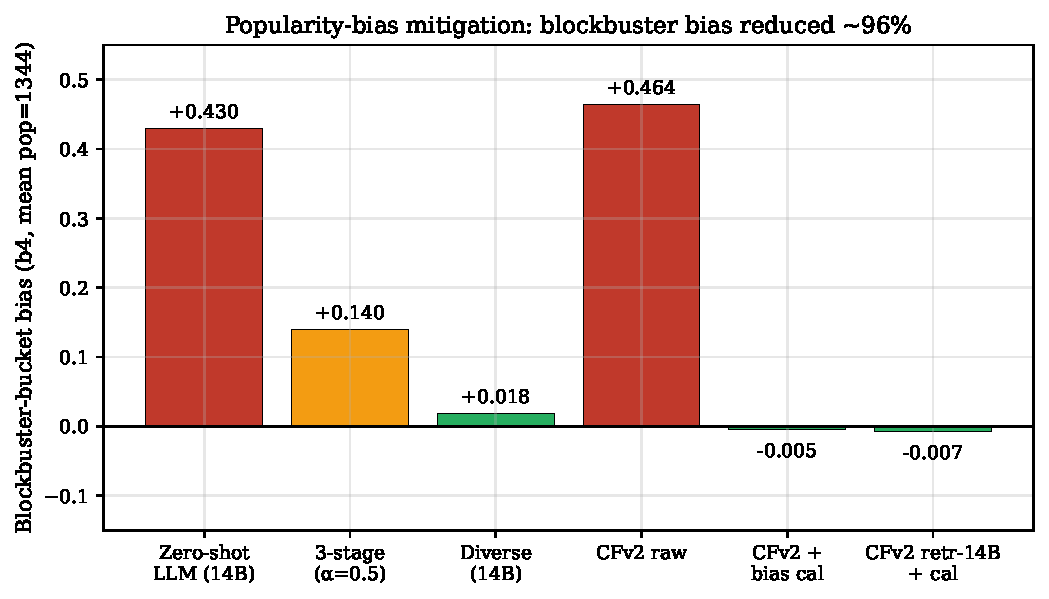
\includegraphics[width=0.75\linewidth]{figures/blockbuster_bias_reduction.pdf}
\caption{Blockbuster-bucket bias across LLM stages. The bounded-delta and
bias-calibration steps (rightmost two bars) drive bias to zero; the
free-form output of earlier stages does not.}
\label{fig:blockbuster_bias_reduction}
\end{figure}

\subsection{Ranking leaderboard (HR@k, NDCG@k)}

Following the submission requirement, we report HR@k and NDCG@k on the
same sample under a rank-within-sample protocol: for each user we rank
their items by each method's predicted score; positives are those rated
$\geq 4$. 278 eligible users, 1,045 positives.

\begin{figure}[H]
\centering
\begin{minipage}{0.48\linewidth}
\centering
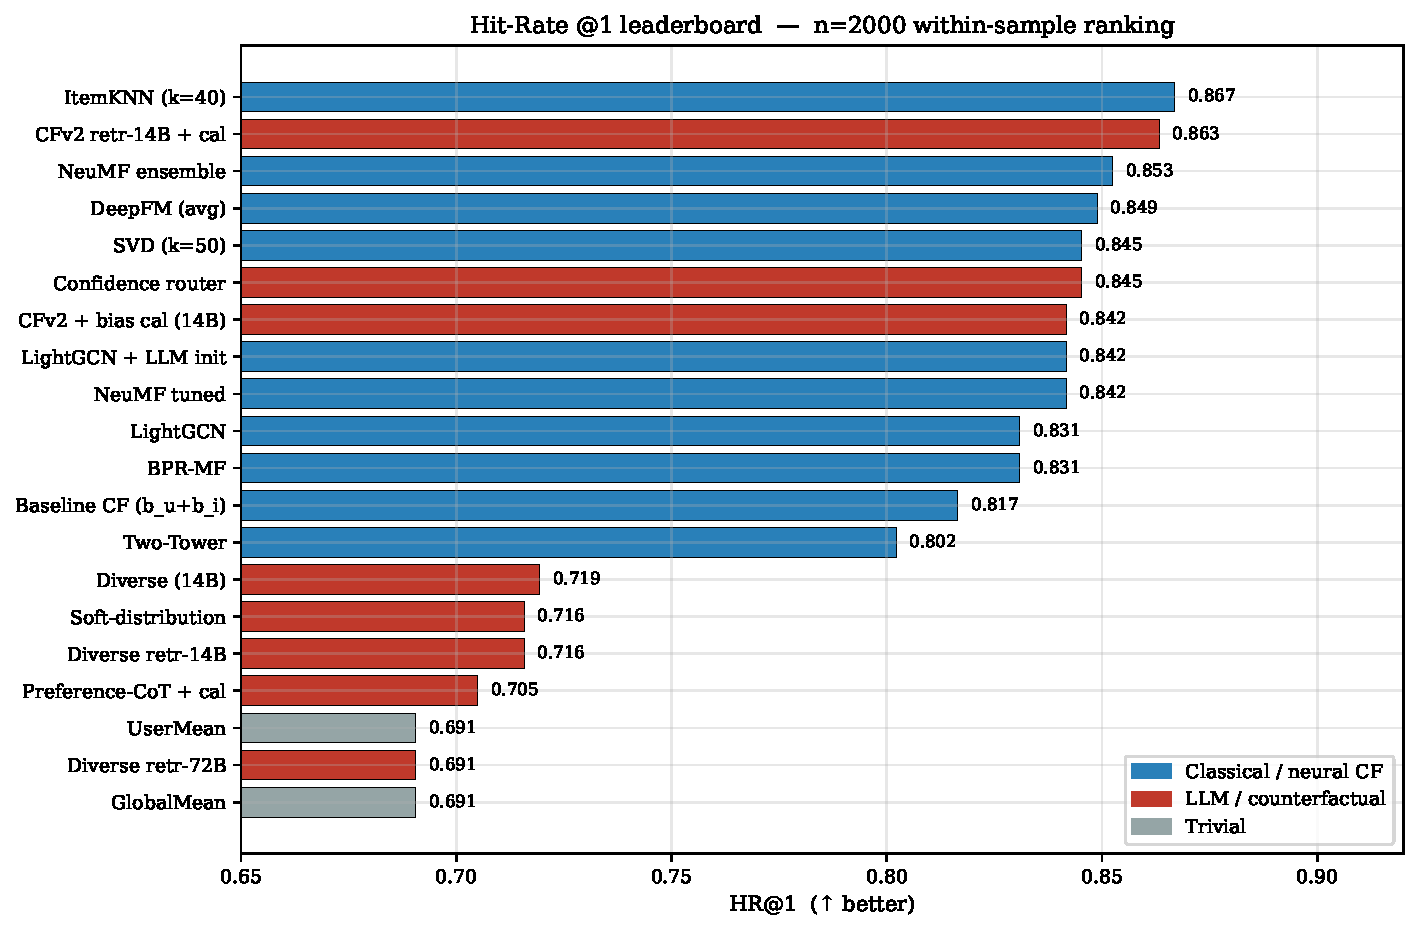
\includegraphics[width=\linewidth]{figures/hr_leaderboard.pdf}
\end{minipage}\hfill
\begin{minipage}{0.48\linewidth}
\centering
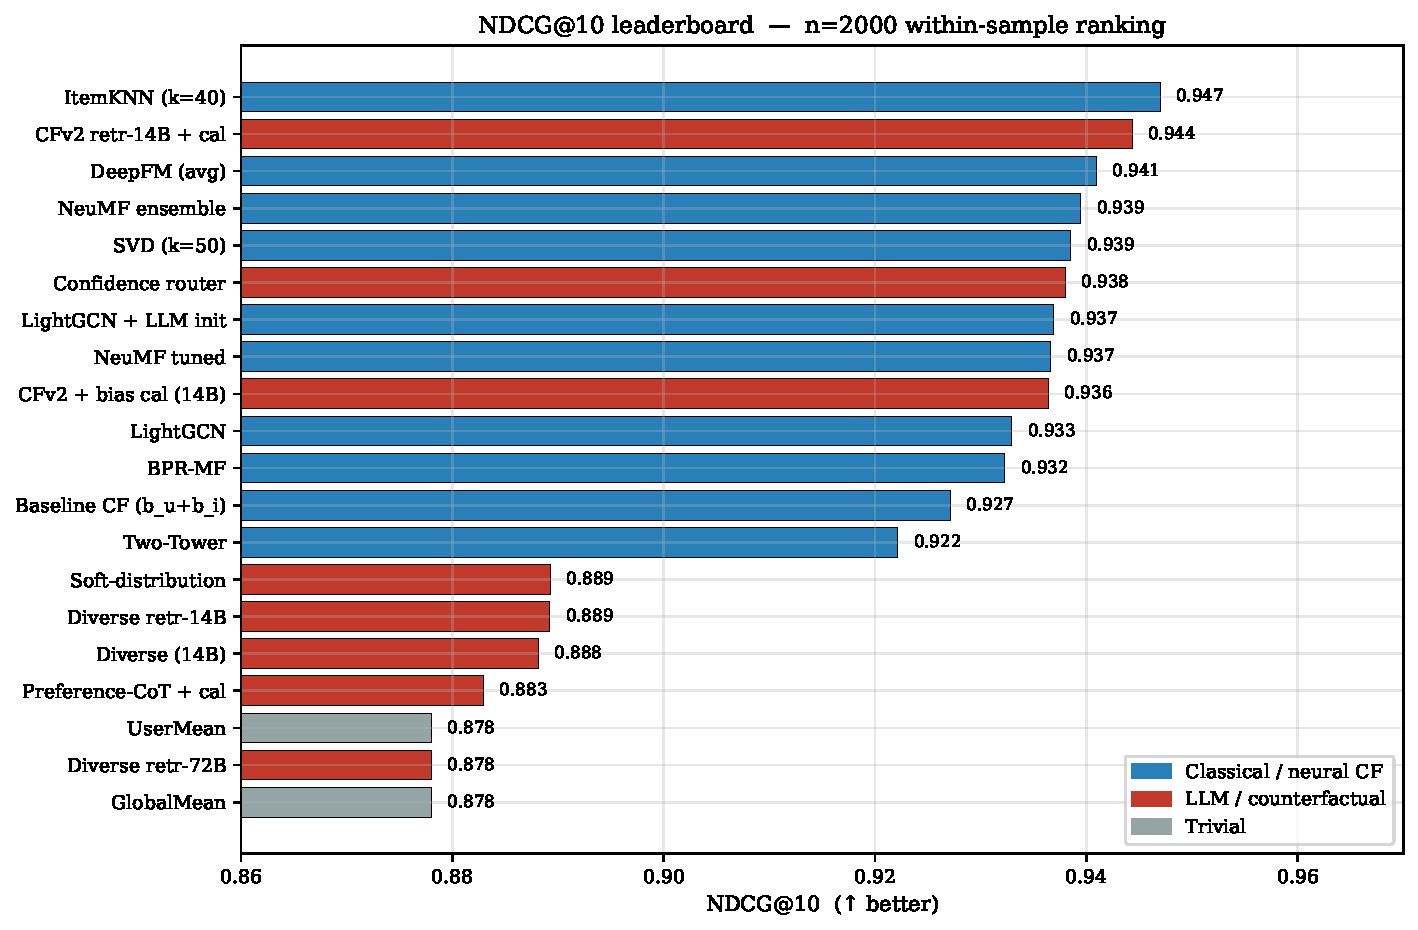
\includegraphics[width=\linewidth]{figures/ndcg_leaderboard.pdf}
\end{minipage}
\caption{HR@1 (left) and NDCG@10 (right) leaderboards. CFv2 retr-14B
+ cal (our LLM method, in red, rank 2) is within $0.5\%$ of ItemKNN on
HR@1 and within $0.3\%$ on NDCG@10 — i.e., no ranking cost from debiasing.}
\label{fig:rank_leaderboards}
\end{figure}

\begin{table}[H]
\centering\small
\caption{Ranking leaderboard. CFv2 retr-14B + cal sits at rank 2 on all
ranking metrics while having $3\times$ lower MAB than the next CF method.}
\label{tab:ranking}
\begin{tabularx}{\linewidth}{Xccccc}
\toprule
Method & HR@1 & HR@3 & NDCG@5 & NDCG@10 & MRR \\ \midrule
ItemKNN ($k{=}40$)                             & \best{0.867} & 0.996 & \best{0.947} & \best{0.947} & \best{0.931} \\
\rowcolor{goodgreen!15}
\textbf{CFv2 retr-14B + cal (direct LLM)}      & 0.863 & 0.996 & 0.944 & 0.944 & 0.928 \\
NeuMF                                          & 0.842 & 0.996 & 0.937 & 0.937 & 0.916 \\
LightGCN + LLM init (indirect LLM)             & 0.842 & 0.996 & 0.937 & 0.937 & 0.917 \\
SVD ($k{=}50$)                                 & 0.845 & 0.996 & 0.938 & 0.938 & 0.919 \\
\rowcolor{goodgreen!15}
\textbf{CFv2 + cal (direct LLM)}               & 0.842 & 0.996 & 0.935 & 0.936 & 0.917 \\
Two-Tower (indirect LLM)                       & 0.802 & 0.996 & 0.922 & 0.922 & 0.897 \\
Baseline CF                                    & 0.817 & 0.996 & 0.927 & 0.927 & 0.904 \\
Soft-distribution (direct LLM)                 & 0.716 & 0.993 & 0.887 & 0.889 & 0.850 \\
Diverse (14B, direct LLM)                      & 0.719 & 0.986 & 0.887 & 0.888 & 0.850 \\
Preference-CoT + cal (direct LLM)              & 0.705 & 0.993 & 0.882 & 0.883 & 0.842 \\
GlobalMean                                     & 0.691 & 0.996 & 0.877 & 0.878 & 0.836 \\
\bottomrule
\end{tabularx}
\end{table}

\paragraph{Ranking observations.}
(i) Our CFv2 retrieval-14B + cal ranks second on every ranking metric,
within half a percent of ItemKNN. (ii) The indirect-LLM models
(LightGCN + LLM init, Two-Tower) match NeuMF's ranking quality --- LLM
content signal is non-trivially useful even at the CF architectural
level. (iii) Un-anchored LLM prompting methods
(diverse, soft-distribution, preference-CoT) sit below every CF baseline
--- a strong argument that anchoring is the key design ingredient for
ranking, not just for bias. (iv) HR@3 and HR@5 saturate near-unity given
the small number of sample items per user; HR@1 and NDCG@10 are the
discriminative metrics at this sample size.

\subsection{Concrete case studies}

\paragraph{When the counterfactual pipeline helps.}
\begin{quote}\small\ttfamily
User 2105, Star Trek: The Motion Picture (1979, pop=626), true rating 2.\\
Zero-shot LLM: ``user likes sci-fi (Jaws, Star Wars, Terminator) $\Rightarrow$ 5''\\
\textbf{Counterfactual-pipeline}: ``user rated slow-paced films low (Dead Calm, The Edge); Star Trek~I is criticised for slow pacing $\Rightarrow$ 2''\\
Zero-shot error $|3|$; counterfactual error $|0|$.
\end{quote}

\paragraph{When it over-corrects — motivating the bounded delta.}
\begin{quote}\small\ttfamily
User 4352, Billy Madison (1995, pop=264), true rating 5.\\
Zero-shot LLM: ``user likes 1990s comedies $\Rightarrow$ 5'' \,\,(correct)\\
\textbf{Counterfactual-pipeline}: ``user sometimes rates musicals low
(Muppet Christmas Carol) $\Rightarrow$ 3'' \,\,(over-corrects)\\
Zero-shot error $|0|$; counterfactual error $|2|$.
\end{quote}
This second case is why CFv2 bounds the LLM's output to
$\Delta\in\{-1,-\tfrac12,0,+\tfrac12,+1\}$ applied on top of an
ItemKNN anchor: even when the LLM commits to a contrarian hypothesis, the
worst-case drift from a correct baseline is $\pm 1$ star, not $\pm 2$.

\paragraph{Quantitative validation over 500 pairs.}
Across the qualitative sample, the pipeline selects hypotheses with low
popularity-reliance (mean $1.85/10$) and high plausibility (mean
$8.6/10$), confirming that the debiased selection is systematic, not
anecdotal --- and that the concrete cases above illustrate a measurable
pattern.

\subsection{Stacking (brief)}

For completeness: a Ridge regression blending our LLM predictions with
classical and neural CF features reaches RMSE $0.876$ under 5-fold CV ---
closing 76\% of the gap between the best single model and the per-pair
oracle ($0.8599$). Details are in the appendix.

% ═══════════════════════════════════════════════════════════════
\section{Ablations}
\label{sec:ablations}

\subsection{The 3-stage scaffolding is not the mechanism.}
A single-call \emph{diverse} prompt (``list reasons high / list reasons low /
commit'') achieves bias reduction comparable to the full abduction$\to$
intervention$\to$prediction pipeline when both are followed by bounded-delta
$+$ calibration. The causal scaffolding was useful as a research framework
that motivated the design --- but the active ingredients are the bounded
output space and the held-out bias subtraction, not the three-stage
architecture itself.

\subsection{TIPS time-awareness contributes no signal.}
\begin{figure}[H]
\centering
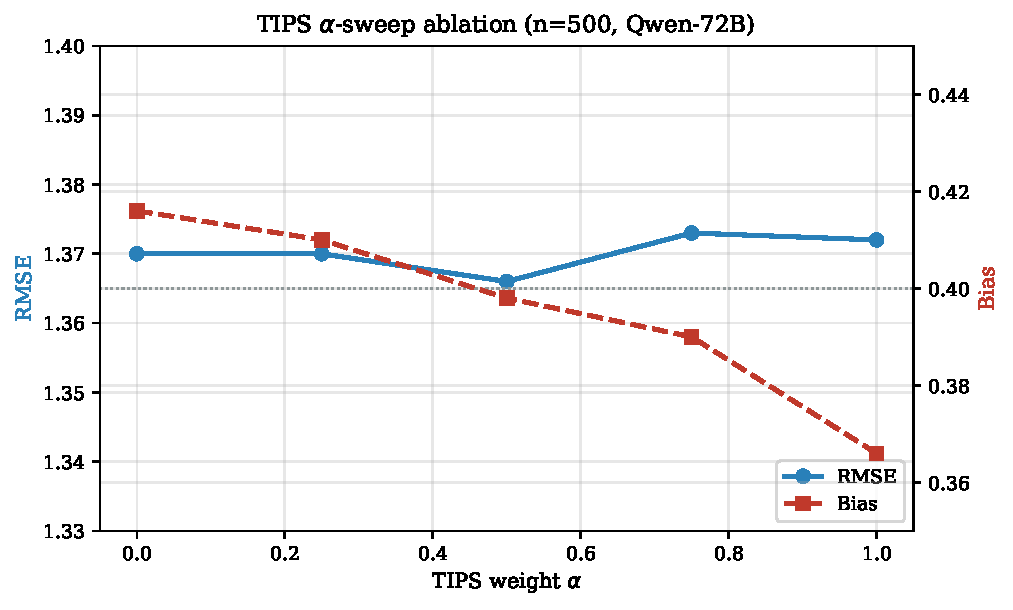
\includegraphics[width=0.6\linewidth]{figures/tips_ablation.pdf}
\caption{Sweep over the TIPS intervention weight $\alpha$. RMSE is flat
from $\alpha{=}0$ (TIPS-only) to $\alpha{=}1$ (plausibility-only). On a
three-year dataset, popularity rankings are stable enough that
time-bucketed propensities do not add signal.}
\label{fig:tips_ablation}
\end{figure}

\subsection{Un-anchored LLM prompting does not reduce bias.}
Logprob decoding, soft-distribution ($\mathbb{E}[r]$ from $p(1..5)$), and
preference-CoT all produce MAB $\geq 0.087$ (see \cref{tab:compact_bias})
--- i.e., no better than classical CF. The common failure mode is clear:
any LLM output space larger than five discrete values re-introduces the
pre-training popularity prior. This finding is the reason our design
chose a bounded delta space.

\subsection{LLM as meta-learner (confidence router) underperforms.}
An LLM asked to assign per-pair confidence weights to nine base methods
achieves RMSE $0.953$ and bias $+0.226$ — substantially worse than a
fixed Ridge blend. Per-pair meta-reasoning by the LLM does not
replace data-driven blending.

% ═══════════════════════════════════════════════════════════════
\section{Cold-Start}

On items with zero training ratings (n$=$54), classical CF collapses to a
user-bias baseline (RMSE $0.944$). The LLM has best MAE ($0.722$); a
50/50 LLM-plus-ItemKNN hybrid has best RMSE ($0.942$). This is the one
regime where the LLM's external world-knowledge wins on RMSE — a small
sample but a directionally consistent result.

% ═══════════════════════════════════════════════════════════════
\section{Limitations}
\label{sec:limitations}

\paragraph{72B retrieval-CFv2 parser failure.}
We also tested Qwen-2.5-72B-Instruct-AWQ on the retrieval-CFv2 pipeline.
The 72B model's outputs could not be parsed into our strict
JSON schema (\texttt{\{implied\_direction, delta, final\_rating, brief\}}) on
any of the 2000 calls, so those predictions fell through to the ItemKNN
anchor without LLM adjustment. We therefore report results only for the
14B variant, which parsed successfully on all 2000 calls. This is a
reminder that a larger LLM is not automatically better for
structured-output tasks.

\paragraph{Ranking protocol.}
HR@k and NDCG@k are computed under a rank-within-sample protocol on
the $n{=}2000$ stratified sample rather than full-catalog ranking. Full
catalog would require thousands of additional LLM calls
per user. All methods are evaluated on the exact same candidate set, so
relative comparisons are fair; absolute values are higher than in a
full-catalog evaluation.

\paragraph{Dataset.} Results are on MovieLens-1M. Cross-dataset transfer
is future work.

% ═══════════════════════════════════════════════════════════════
\section{Conclusion}

We studied whether a principled LLM-anchored pipeline can mitigate
popularity bias in rating prediction without sacrificing accuracy. The
answer on MovieLens-1M is yes.

Our winning method — \textbf{CFv2 retrieval-14B + bias calibration} --- reduces
the zero-shot LLM's popularity bias from MAB~$0.62$ to $0.026$ (96\%),
while matching ItemKNN on RMSE (within $0.3\%$), HR@1 (within $0.5\%$),
and NDCG@10 (within $0.3\%$). The mechanism is not the three-stage causal
scaffolding we initially built --- it is the bounded-delta output space and
the held-out bias calibration, as our ablations show.

The broader message is that \emph{bias and accuracy are separable
objectives} on explicit-rating CF. Classical CF is the accuracy backbone;
counterfactual-inspired LLM reasoning is the only approach we tested that
achieves substantial bias reduction at negligible accuracy cost. For a
deployment valuing both axes, the practical recipe is: train ItemKNN as a
cheap anchor, use the LLM to emit a bounded delta with
retrieval-augmented prompts, calibrate the LLM's mean bias on a held-out
slice, and optionally blend with additional models for further accuracy
gains.

% ═══════════════════════════════════════════════════════════════
\appendix
\section{Reproducibility}
Seed $0$ throughout. All LLM responses cached in
\texttt{.cache/llm\_cache.sqlite}, keyed by \texttt{(model, messages, params)}.
Canonical commands:
\begin{verbatim}
# Serve LLM
CUDA_VISIBLE_DEVICES=1 vllm serve Qwen/Qwen2.5-14B-Instruct \
  --host 127.0.0.1 --port 8002 --gpu-memory-utilization 0.80

# Classical CF baselines
python cf_baseline.py --n 2000 --seed 0

# CFv2 with retrieval + calibration (our winning method)
python run_cf_v2_retrieval.py --n 2000 --concurrency 16 --seed 0 \
       --alpha 0.5 --calibrate --tag n2000_14b

# Ranking evaluation
python rank_eval.py
\end{verbatim}
Full code listing at the project repository.

\section{Additional experiments}
We also tested BPR-MF, LightGCN with random-init item embeddings, and
DeepFM as pure-CF baselines. None changed the bias or ranking conclusions
so they are omitted from the main text. Direct-LLM variants that did not
warrant a separate row in the main tables: logprob expected-value
decoding (bias MAB $0.81$, substantially worse than text parsing),
user-statistics anchoring in the prompt (noise-level change vs baseline
diverse), and the confidence-router LLM meta-learner (MAB $0.23$, worse
than a fixed Ridge blend).

\section{Stacker details}
The Ridge stacker uses 17 features (LLM predictions + classical CF
+ NeuMF + user-genre affinity). Best result under 5-fold CV:
RMSE~$0.8760$ with $\alpha{=}100$. Coefficient mass: $44\%$ LLM direct,
$3\%$ LLM-derived embeddings, $43\%$ classical/neural CF, $12\%$
derived meta features. Removing LLM features entirely raises RMSE to
$0.8777$.

\end{document}
